\chapter{Classification I: Entscheidungsbaum und Random Forest}

\section{Entscheidungsbaum}

\begin{mydefinition}
    Ein \textbf{Entscheidungsbaum} teilt Daten schrittweise auf. Jede Verzweigung stellt eine Frage
    (z.\,B. \enquote{Lernzeit > 6h?}) und führt zu einer Entscheidung.
\end{mydefinition}

\begin{figure}[H]
    \centering
    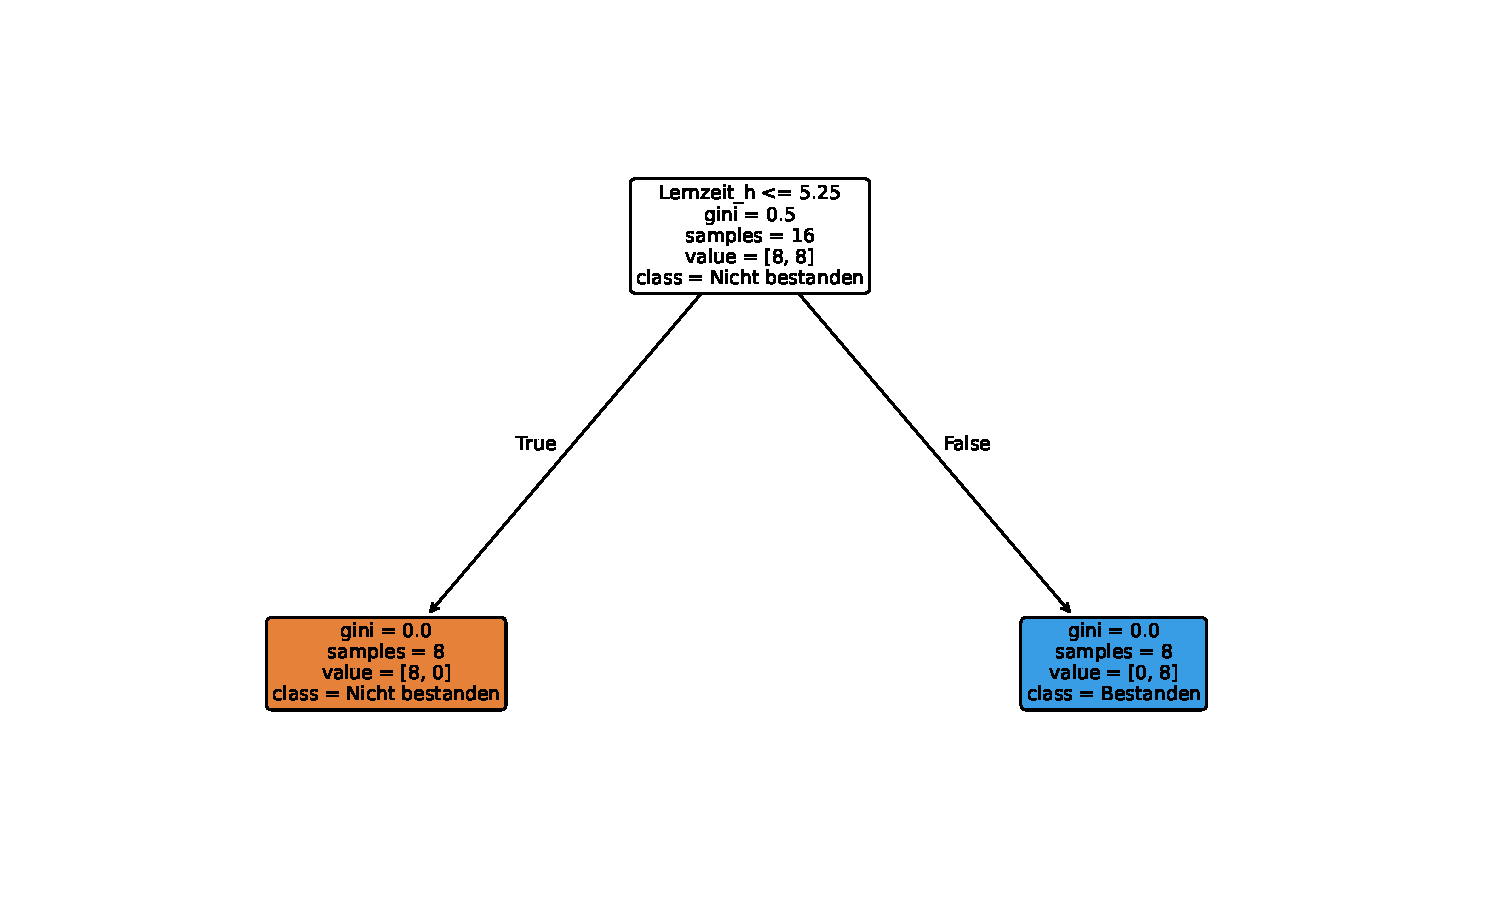
\includegraphics[width=0.8\textwidth]{Grundlagen_Info/15_KI_und_Algorithmen/Figures/decision_tree_structure.pdf}
    \caption{Beispiel eines Entscheidungsbaums}
    \label{fig:tree-15}
\end{figure}

\begin{myexercise}[Baum lesen]
    Betrachten Sie \cref{fig:tree-15}:
    \begin{enumerate}
        \item Welche Eigenschaft wird an der Wurzel geprüft?
        \item Geben Sie einen möglichen Pfad bis zu einer Klasse an.
        \item Nennen Sie einen Vorteil von Entscheidungsbäumen im Unterrichtskontext.
    \end{enumerate}
\end{myexercise}

\begin{myremark}[Notebook]
    Praktische Umsetzung inkl. Übungen:
    \href{\notebookbaseurl01_Entscheidungsbaum_Classification.ipynb}{\texttt{01\_Entscheidungsbaum\_Classification.ipynb}}
\end{myremark}

\section{Random Forest}

\begin{mydefinition}
    Ein \textbf{Random Forest} kombiniert viele Entscheidungsbäume. Die Endentscheidung entsteht
    über Mehrheitsabstimmung der einzelnen Bäume.
\end{mydefinition}

\begin{figure}[H]
    \centering
    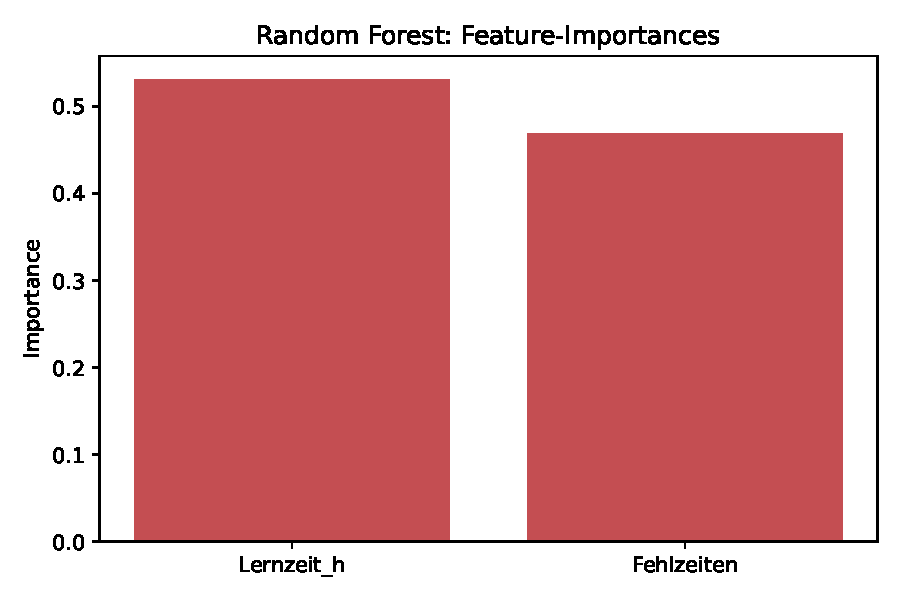
\includegraphics[width=0.72\textwidth]{Grundlagen_Info/15_KI_und_Algorithmen/Figures/random_forest_feature_importance.pdf}
    \caption{Feature-Importances eines Random-Forest-Modells}
    \label{fig:rf-importance-15}
\end{figure}

\begin{myexercise}[Vergleich Baum vs. Wald]
    Diskutieren Sie in Zweiergruppen:
    \begin{itemize}
        \item Warum kann ein einzelner Baum schnell \enquote{auswendig lernen}?
        \item Warum ist ein Wald oft robuster?
        \item Welche Nachteile hat der Random Forest gegenüber einem einzelnen Baum?
    \end{itemize}
\end{myexercise}

\begin{mychallenge}[Hyperparameter verstehen]
    Recherchieren und erklären Sie kurz:
    \begin{itemize}
        \item \texttt{n\_estimators}
        \item \texttt{max\_depth}
        \item \texttt{min\_samples\_leaf}
    \end{itemize}
    Wie beeinflussen diese Parameter die Modellkomplexität?
\end{mychallenge}

\begin{myremark}[Notebook]
    Praktische Umsetzung inkl. Übungen:
    \href{\notebookbaseurl02_Random_Forest_Classification.ipynb}{\texttt{02\_Random\_Forest\_Classification.ipynb}}
\end{myremark}
